%!TEX root = ../main.tex

\chapter{Introduction} % (fold)
\label{cha:introduction}

%************************************
% 1 Introduction
% 1.1 Contextualization
% 1.2 Motivation
% 1.3 Objectives
% 1.4 Methodology
% 1.5 Document Structure
%************************************

This chapter provides an overview of the context, motivation, objectives, and methodology of this dissertation. It begins by discussing the applications of all-digital \gls{TDC} and providing a brief review of the different platforms that could be used to develop such system. The motivation for the project is then presented, outlining the problem that the author seeks to address. To ensure that all of the planned results are achieved, the project objectives and methodology must be established. Finally, this chapter concludes with a description of the dissertation document structure.

\section{Contextualization} % (fold)
\label{sec:contextualization}

Precise measurement of time elapsed between two event or time pulses is an essential requirement for many science and engineering applications. \Acrlongpl{TDC} are extremely high-precision stopwatches which convert time domain information into a digital representation. They represent the fundamental building blocks between the continuous time domain and the digital world.

All-digital \glspl{PLL} were the first \gls{TDC} application. \glspl{PLL} are feedback systems that generate signals phased locked with external input signals where a \gls{TDC} serves as phase detector \citep{pll}. \glspl{TDC} are used in applications where precise time interval measurements are required. They have been applied for a long time in the nuclear and particle high-energy physics field \citep{physics}. Other applications cover space sciences \citep{space_sciences}, biomedical applications, such as positron emission tomography and \gls{FLIM} \citep{flim}, and \gls{ToF} measurements thus \gls{LiDAR} systems \citep{lidar}.

Among other applications, \gls{LiDAR} imaging systems play a key role in autonomous vehicles. The Society of Automotive Engineers currently defines six levels of driving automation ranging from Level 0 (fully manual) to Level 5 (fully autonomous) \citep{sae_av}. These levels have been also adopted by the U.S. Department of Transportation. Although being relatively new in automotive markets, the vehicle surrounding mapping advantages offered by \gls{LiDAR}, when compared to other technologies, have propelled massive innovations. \gls{LiDAR} imaging systems are a novel type of sensor which enable complete three-dimensional perception of the environment, and not just the two-dimensional projection obtained from a camera. A combination of radar, video cameras, and \gls{LiDAR} with deep learning procedures is the most likely solution for a vast majority of cases \citep{lidar_ov}. Thus, \gls{LiDAR} will be at the core of this revolution.

\Gls{LiDAR} sensors bounce pulses of light off the car’s surroundings to measure distances, detect road edges, and identify lane markings \citep{lidar_ov}. This working principle is illustrated in Figure \ref{fig:lidar}. Companies previously established in the field are being acquired by large industrial corporations, mainly from the automotive industry. This activity is due to the lack of an adequate solution in all aspects for \gls{LiDAR} image systems for automotive either because performance, lack of components, industrialization, or cost issues \citep{lidar_ov}.

\begin{figure}[ht!]
    \centering
    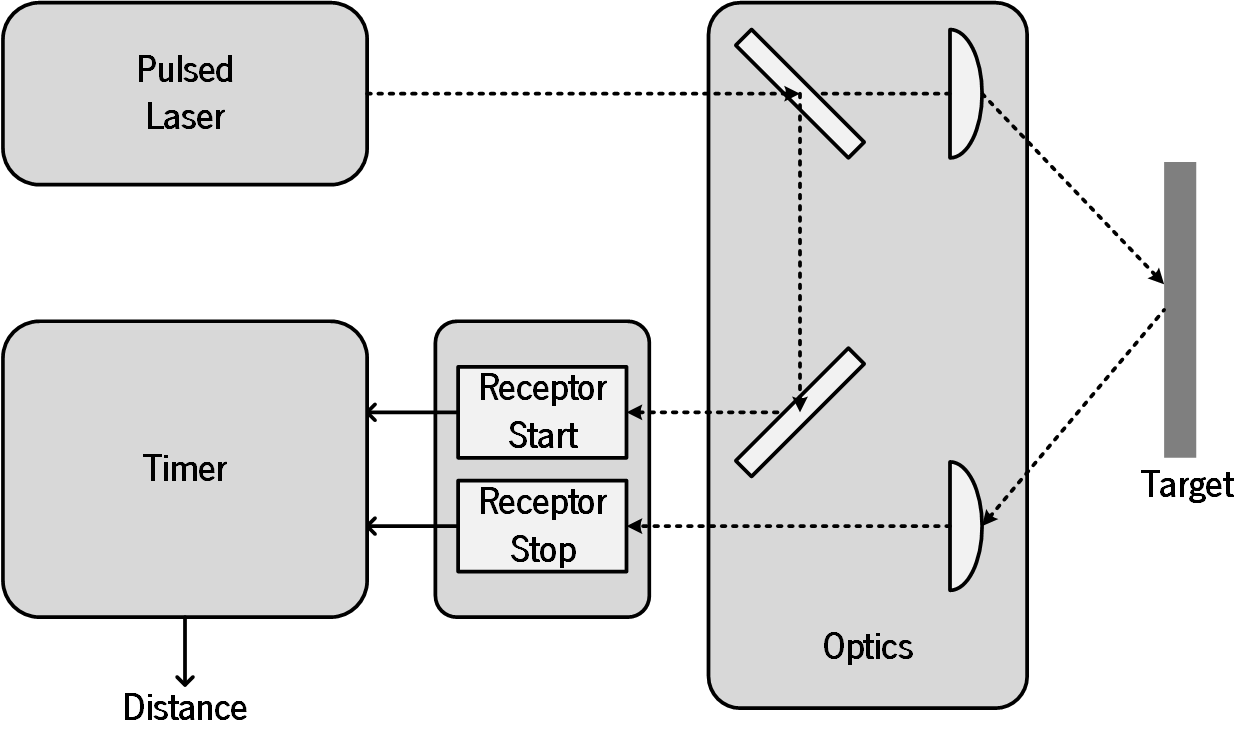
\includegraphics[width=.5\textwidth]{img/01_introduction/LiDAR.png}
    \caption{Pulsed time-of-flight measurement principle (adapted from \citep{lidar_ov}).}
    \label{fig:lidar}
\end{figure}

\Glspl{TDC} can be divided into two categories based on their operating principles. Analog \glspl{TDC} convert a time interval into a voltage, which is then digitized by an \gls{ADC}. These \glspl{TDC} have good resolution and linearity, but they also have high-power dissipation, large size, low scalability, and high susceptibility to noise. All-digital \glspl{TDC}, on the other hand, can simultaneously achieve high resolution and wide dynamic range, with small area and low power dissipation \citep{cheng_ov}. Due to these advantages, all-digital \glspl{TDC} are currently the most appealing approach to most applications.

All-digital \glspl{TDC} are primary implemented either using \gls{ASIC} or \gls{FPGA} devices. The requirements for price, reproducibility, and suitability for mass production differ depending on the application. Over the years, the performance gap between \glspl{FPGA} and \glspl{ASIC} has been narrowed due to the constant development of \gls{FPGA} technology, including the fabrication process and development tools technology \citep{FPGA_ASIC}. This has made \glspl{FPGA} a viable option for final products, rather than just prototypes. The high performance, lower development cost and time to market make \gls{FPGA}-based systems appealing to different applications, including \glspl{TDC}. As a result, \gls{FPGA}-based \glspl{TDC} have become increasingly popular in recent years.

% section contextualization (end)

\section{Motivation} % (fold)
\label{sec:motivation}

The main key performance indicators of \glspl{TDC} are the measurement range, resolution and precision, nonlinearities, dead-time, power consumption and resources usage. Much research has focus on increasing resolution of \glspl{TDC}; however, nonlinearities can have a direct impact on the overall system precision. \Gls{PVT} variations are one of the main causes of \gls{TDC} nonlinearities. A high-stability power supply and temperature control equipment can be used to control voltage and temperature fluctuations, however this increases system cost and complexity. Therefore, a special correction strategy is needed to compensate for \gls{PVT} variations without affecting \gls{TDC} normal operation. This dissertation aims to develop such a calibration.

% section motivation (end)

\section{Objectives} % (fold)
\label{sec:objectives}

The goal of this dissertation is to develop a high-resolution \gls{TDC} with 20~ps resolution and 20~ps precision that is not heavily influenced by \gls{PVT} conditions. To achieve this, several objectives must be pursued:

\begin{itemize}
    \item Review the state-of-the-art in time interval measurement systems;
    \item Develop a high-performance time interval measurement system;
    \item Develop and integrate a calibration system to compensate \gls{PVT} variations;
    \item Evaluate the performance of the developed architecture to understand its viability in different scenarios and how should the \gls{ToF} measurement systems should be characterized;
    \item Evaluate the proposed architecture and compare it to the existing state-of-the-art \glspl{TDC}.
\end{itemize}

% section objectives (end)

\section{Methodology} % (fold)
\label{sec:methodology}

To focus and guide the activities involved in the research process that would enable the attainment of the proposed objectives, several research methodologies will be adopted during this dissertation:

\begin{itemize}
    \item \textbf{State-of-the-art of \gls{TDC}:} A review of the state-of-the-art of interval measurement systems will be performed to understand the different type of architectures that are being implemented and their typical performances. This review will focus on FGPA-based \glspl{TDC}, as they are the target application for this research.

    \item \textbf{Study the \gls{FPGA} development framework:} To develop time interval measurement systems with a resolution under the clock frequency, a deep understanding of how the development frameworks are configure is required, as well as advanced knowledge of the \gls{FPGA} platform being used. A study of the Xilinx Vivado framework will be conduct to learn how to avoid automatic optimizations on parts of the design and force the framework to generate specific hardware directly mapped to the \gls{FPGA} configurable blocks. This study will also explore how manual placement and routing can be used to improve  the overall performance of the time interval measurement system. In addiction, a study of the available \gls{FPGA} platform resources and their configuration will be performed.

    \item \textbf{Evaluation \gls{FPGA}-based \glspl{TDC}:} The main metrics that need to be consider for proper \gls{TDC} evaluation will be characterized. This include determining which tests need to be performed and how to conduct them. Code density tests to evaluate \gls{TDC}’s mean resolution and nonlinearities, performance measurements to obtain the \gls{TDC}’s precision and tests to analyze the \gls{TDC}'s performance variation with temperature will be the main focus of the evaluation.

    \item \textbf{Development of \gls{FPGA}-based \gls{TDC} prototype:} An architecture will be developed targeting a \gls{FPGA} device with the goal of achieving the highest possible resolution.

    \item \textbf{Development of calibration system:} A calibration system will be developed to compensate \gls{PVT} variations.

    \item \textbf{Characterization and integration of the developed \gls{TDC}:} To compare the developed \gls{TDC} with the existing implementations, a set of tests will be performed to evaluate the \gls{FPGA}-based \gls{TDC}. The architectures will be compared using the main \gls{TDC} performance metrics.
\end{itemize}

% section methodology (end)

% chapter introduction (end)
